\section{Definição da Solução}

\subsection{Escopo}
Nesta seção serão apresentados as visões da construção do projeto.

\subsubsection{Visão Geral da Estrutura}
Nesta seção foram levantados as decisões dos aspectos estruturais do projeto. A estrutura do produto a ser desenvolvido envolve critérios que são específicos do contexto deste projeto. Os critérios afetam diretamente o diferencial de mercado além de cumprir com questões legais. Os critérios foram divididos em dois grupos: \textbf{estrutural} e \textbf{material}.

\begin{enumerate}
  \item \textbf{Estrutura} 
\end{enumerate}

Ao desenhar a estrutura do Robô foi identificado que deve-se levar em consideração os seguintes aspectos: melhor identificação da criança com o equipamento, segurança;

\begin{itemize}
  \item \textbf{Melhor identificação da criança com o equipamento}
  \begin{itemize}
    \item \textbf{Cor}: Pagnan (2009) Afirma que a cor exerce uma ação tríplice: a de impressionar a de expressar e a de construir, portanto o aparelho deve apresentar coloração atrativa,  e também faz uma relação entre as cores e as respectivas características psicológicas e simbólicas, para os propósitos do trabalho selecionamos duas cores: \textbf{azul}, exerce apelo intelectual, simbolizando a inteligência e raciocínio; \textbf{vermelho}, estimulante e dinâmica é a cor preferida da criança.
    \item \textbf{Aparência}: Quanto a aparência ela deve ter aparência agradável, intuitiva e associado a elementos que o usuário conheça e se identifique, as formas especuladas são veículos e elementos de filmes desenhos e etc.
  \end{itemize}
\end{itemize}

\begin{itemize}
  \item \textbf{Segurança} O produto oferecido não deve apresentar nenhum tipo de risco a integridade física da criança, portanto o produto deve possuir design “macio”, não apresentando pontas ou qualquer componente que venha a amplificar um possível tipo de dano causado por contato mecânico.
\end{itemize}

\begin{enumerate}
  \item \textbf{Material} 
\end{enumerate}

Para selecionarmos o material a ser utilizado na estrutura os critérios considerados foram:

\begin{itemize}
  \item \textbf{Segurança} - Nesse aspecto os riscos identificados foram: toxicidade, choque mecânico.
  Segundo a Ficha de informações de segurança do produto químico da The Dow Chemical Company o HDPE não é uma Substância Química Perigosa, classificado pela definição do Padrão OSHA de Comunicação de Perigos, 29 CFR 1910.1200. Ainda segunda a The Dow Chemical Company o contato prolongado não é irritante para a pele e nem a pele absolve de alguma maneira o material, portanto os principais riscos que o material deve apresentar são inerentes a todos os materiais e se devem a choques mecânicos. Esses choques mecânicos podem ser amenizados dependendo do processo de fabricação, que pode ser escolhido para produzir um material mais ‘macio’ e que ao mesmo tempo aguente os esforços mecânicos a qual o robô será submetido.
  \item \textbf{Propriedade Mecânica} - Os principais esforços identificados a qual o robô será submetido foram: queda, peso (devido a objetos em cima do robô), choques com obstáculos.
  Como podemos ver, os esforços a qual o robô vai está submetido são de natureza simples, e não possuem magnitudes elevadas. Portanto (estamos estimando aqui) as propriedades do HDPE listada abaixo, conseguem ser suficientes para garantir a integridade estrutural do robô.
  \begin{figure}[H]
    \centering
    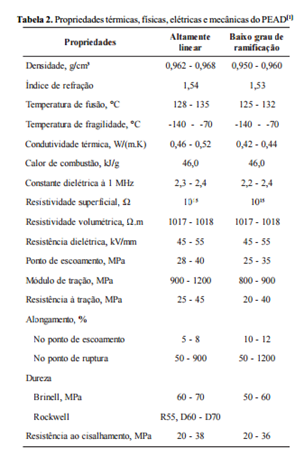
\includegraphics[width=.5\textwidth]{edit/img/especificacao.png}
    \caption{Propriedade do HDPE}
    \label{hdpeprop}
  \end{figure}

  Em comparação com o alumínio que foi o outro material considerado e que é comumente usado nesse tipo de aplicação, essas propriedades validam o uso do HDPE no projeto. O grande diferencial do HDPE foi o preço e a maior facilidade de conformar o material para forma desejada. Segue abaixo uma tabela com as propriedades do alumínio CAST 7000, um dos mais usados para construção de chassi de maquinas no geral:

  \begin{figure}[H]
    \centering
    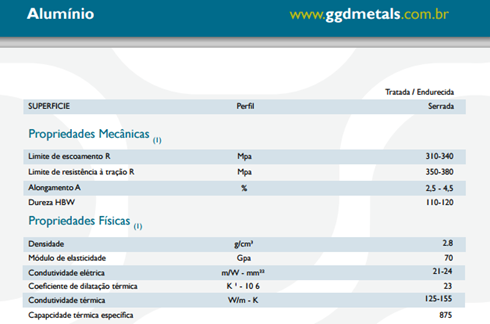
\includegraphics[width=.5\textwidth]{edit/img/especificacao2.png}
    \caption{Propriedades do Alumínio CAST 7000}
    \label{cast7000prop}
  \end{figure}

  \item \textbf{Proteção dos Equipamentos} - Nesse tópico as principais preocupações foram: transferência de calor, condução elétrica. Como podemos ver, o HDPE apresenta as propriedades de condução térmica e elétrica em ordens de grandeza bem menor que a do alumínio. Portanto é o mais indicado nesse quesito.

\end{itemize}

De todos os 3 aspectos considerado o HDPE apresenta vantagens em todos eles portanto a priori é o material que será utilizado na execução do projeto. A massa e dimensões do carrinho ainda não foram especificadas devido a aparência/geometria do mat erial ainda não ter sido escolhida. Por consequência não foi feita completamente a analise estrutural do robô.

\begin{enumerate}
  \item \textbf{Esteira}
\end{enumerate}
A escolha de um sistema de esteiras como forma de locomoção do robô foi devida à possível demanda por mobilidade em diversos ambientes de funcionamento. Estes ambientes podem ser em jardins, parques, um quintal de uma casa.  
O uso de esteiras nesses ambientes de terrenos irregulares garante uma maior área de contato do robô com o chão que permite uma maior tração e consequentemente um maior controle nos pisos naturais \cite{bekker:1956}.
O que foi levado em consideração para escolha do tipo de sistema (roda x esteira) foram as características de Mobilidade, Sobrevivência e Confiabilidade \cite{bekker:1956} A mobilidade seria a facilidade que a esteira teria de se movimentar pelos terrenos de forma rápida e livre, portando a mobilidade seria a característica de liberdade de movimento do sistema. A sobrevivência seria ligada à durabilidade de todo o sistema e em como ele irá reagir durante seu uso nos diversos terrenos.  A Confiabilidade consistiria em como o sistema necessitaria de manutenção e a existência de suprimentos para manutenção. Outro dado levado em consideração foi a quantidade de energia necessária para usar os sistemas, apesar de demandar mais energia para movimentar as esteiras as vantagens sobre as rodas foram decisivas para escolha das esteiras.
O controle de um robô que usa esteiras é mais complexo do que o que usa rodas, mas as vantagens de oferecer maior tração em terrenos irregulares, serem mais robustos e aguentarem maiores impactos foram as características que permitiram a escolha do sistema.

  Raspberry Pi: Devido a sua simplicidade, baixo custo e grande número de recursos, a plataforma raspberry pi será utilizada no processamento dos sensores e de toda a lógica embarcada do robô. É através dele que será realizada a comunicação com o aplicativo de controle, como também a execução das tarefas pelo robô \cite{jornalggn:2013}.

\begin{itemize}
  \item \textbf{Adaptador Wi-fi}: A comunicação entre o robô e o aplicativo será realizada utilizando-se um adaptador wi-fi para raspberry pi. Essa comunicação foi escolhida por suprir as necessidades da aplicação em questão, com um razoável custo monetário.
  \item \textbf{Motor de passo}: Serão utilizados dois motores de passo para realizar a movimentação do robô. Motores de passo são utilizados em aplicações que necessitam movimentos precisos, como controle de velocidade e ângulo de rotação das rodas do robô.
  \item \textbf{Sensores de luz}: Sensores de luz podem ser utilizados como forma de incrementar e auxiliar no que se refere a aplicações relacionadas ao desenvolvimento do raciocínio lógico proposto nesse trabalho.
  \item \textbf{Sensores ultrassom}: Sensores ultrassom serão utilizados no auxílio do controle e lógica da estimativa da distância de possíveis obstáculos na trajetória do robô, esse controle ajudará também no desenvolvimento da lógica condicional que fará parte da estratégia de desenvolvimento do raciocínio lógico proposta no trabalho.
\end{itemize}

\subsubsection{Visão Geral do Controle}

Nesta seção será apresentada a visão geral do sistema de controle do projeto, mostrando como será a interação entre componentes físicos, embarcado, aplicativo mobile e api.
O sistema de controle tem o objetivo de prover a interação entre o usuário e o robô, garantindo a integridade dos comandos e a sua plena execução. A figura \ref{sys:ctlr} mostra um diagrama representando a comunicação entre os principais componentes do sistema.
\begin{figure}[H]
  \centering
  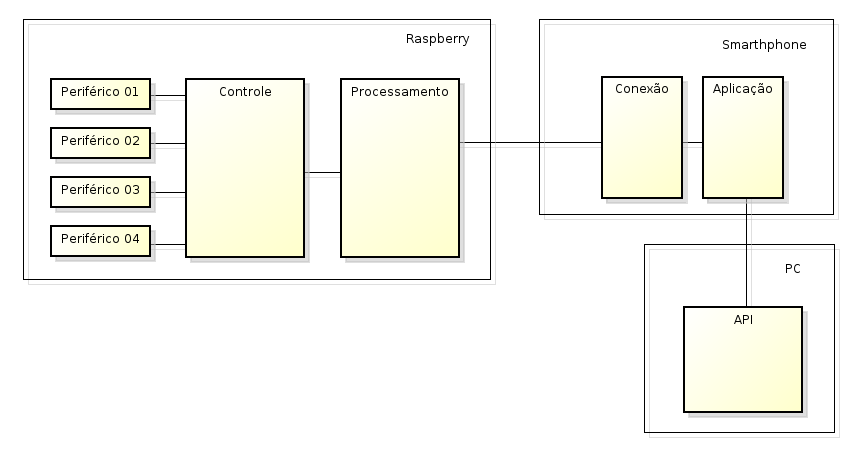
\includegraphics[width=.9\textwidth]{edit/img/visao_geral_controle.png}
  \caption{Diagrama do sistema de controle}
  \label{sys:ctlr}
\end{figure}

\begin{itemize}
  \item \textbf{Periférico}: qualquer componente físico que coleta dados ou realiza alguma ação no ambiente;
  \item \textbf{Controle}: módulo responsável por transferir comandos para os periféricos, sejam de ação ou coleta;
  \item \textbf{Processamento}: módulo responsável por realizar o processamento dos dados recebidos pela aplicação \textit{mobile};
  \item \textbf{Conexão}: módulo responsável por estabelecer e manter a conexão do dispositivo \textit{mobile} com o compenente \textit{rapberry};
  \item \textbf{Aplicação}: aplicativo \textit{mobile} que provê a interface gráfica para comunicação entre usuário e o sistema;
  \item \textbf{API}: módulo para alteração de determinadas partes da aplicação \textit{mobile}.
\end{itemize}
